\newpage
\section{User Interface Design}
\subsection{Homepage}
In both mobile application and browser, from homepage it's possible to move to all functions: login, registration, request and reservation (these two only for users registered as passengers) and Manage work (only for users registered as taxi drivers).
\begin{figure}[H]
\centering
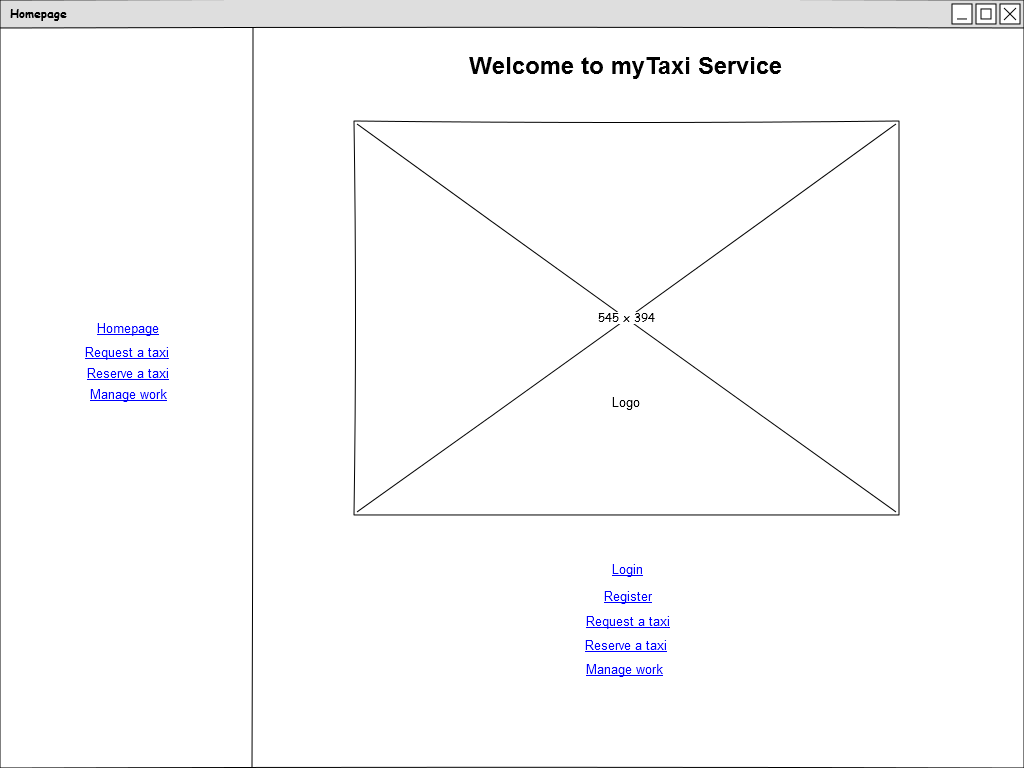
\includegraphics[scale=0.3]{mockups/homepage_web.png}
\caption{Homepage Web Version}
\end{figure}
\begin{figure}[H]
\centering
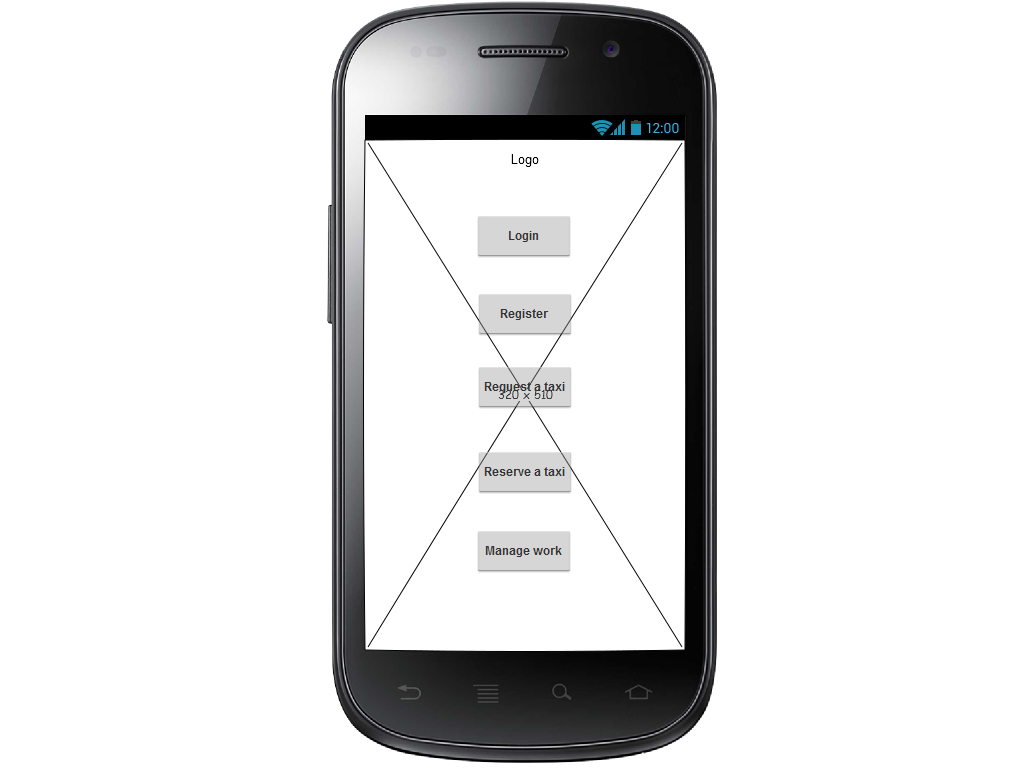
\includegraphics[scale=0.3]{mockups/homepage_mobile.png}
\caption{Homepage Mobile Version}
\end{figure}
\break
\subsection{Registration}
Users can register themselves from this page filling various fields. The majority of these last ones are in common for every person who wants to register, but there is a field reserved to taxi drivers (taxi driver license number) that can be filled only choosing taxi driver, in the web registration page menu, or taxi driver radio in the mobile registration page. \newline Before confirming the registration, it's necessary to accept policies about privacy and use of user's personal details. \newline
From this browser page users can go to homepage and other important pages.
\begin{figure}[H]
\centering
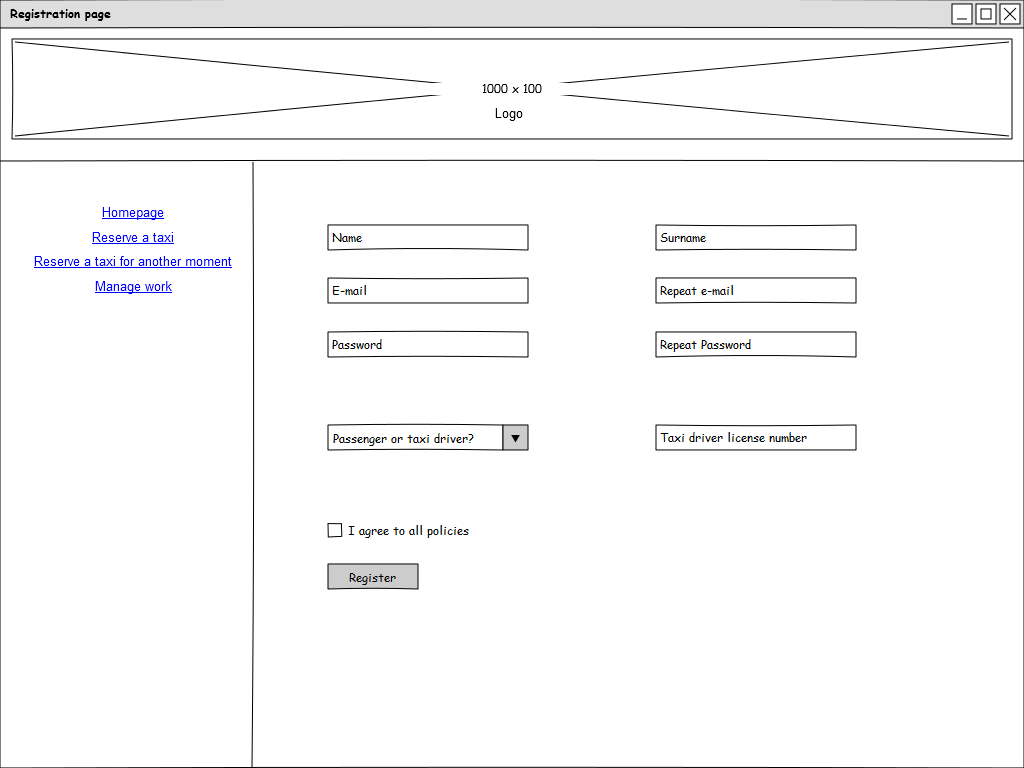
\includegraphics[scale=0.35]{mockups/registration_web.png}
\caption{Registration Web Version}
\end{figure}
\begin{figure}[H]
\centering
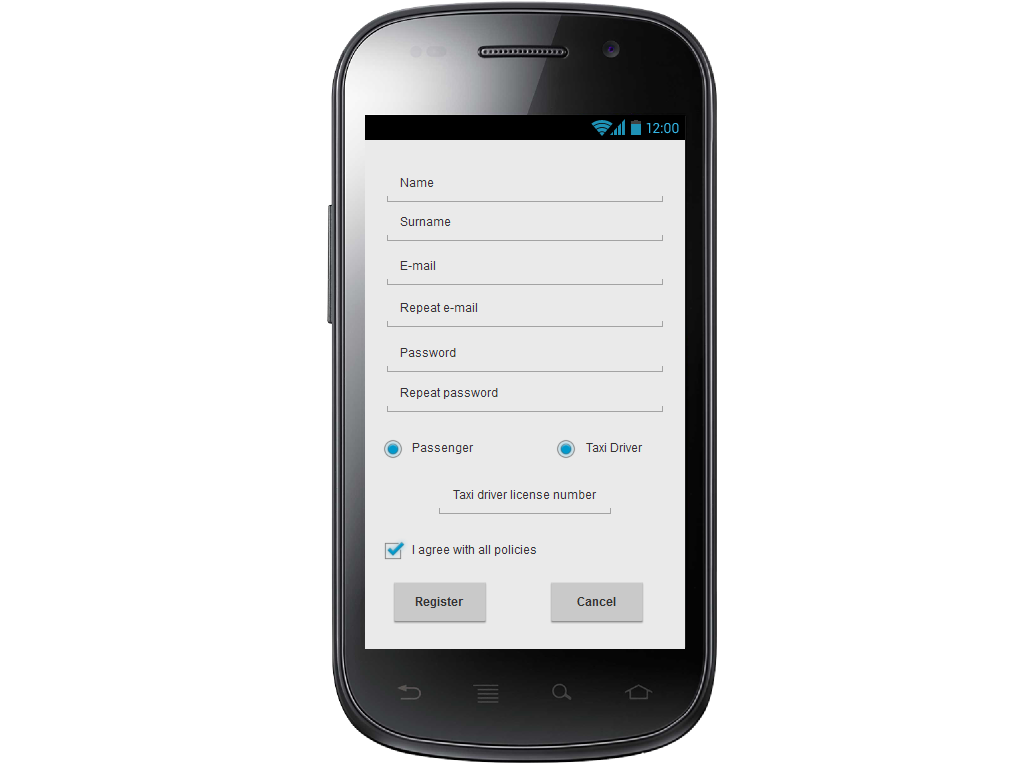
\includegraphics[scale=0.35]{mockups/registration_mobile.png}
\caption{Registration Mobile Version}
\end{figure}
\break
\subsection{Login}
From this page registered users can log in inserting either the registration email or username and the password chosen during registration. \newline If an user forgets his/her password, username or email, it's possible to recover them: a message on the mobile phone or an email is sent to him/her. \newline Also from this browser page users can go to homepage and other important pages. 
\begin{figure}[H]
\centering
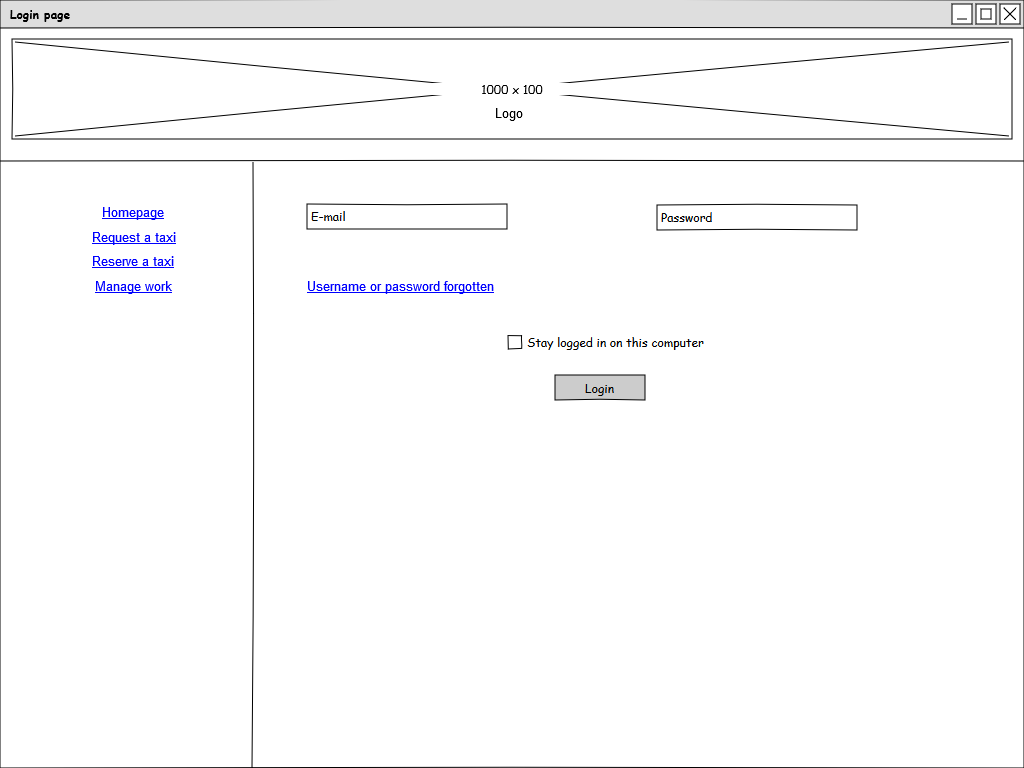
\includegraphics[scale=0.35]{mockups/login_web.png}
\caption{Login Web Version}
\end{figure}
\begin{figure}[H]
\centering
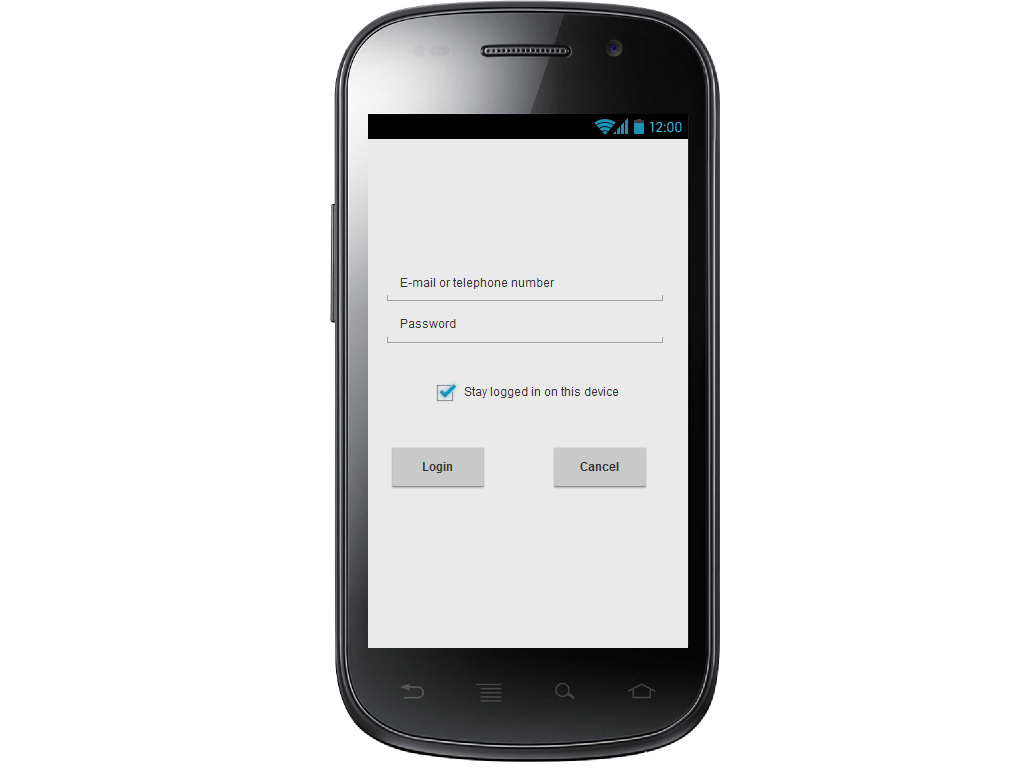
\includegraphics[scale=0.35]{mockups/login_mobile.png}
\caption{Login Mobile Version}
\end{figure}
\break
\subsection{Recovery Password}
In the web version, registered users can recover their username, password and registration e-mail inserting following information. A SMS will send to the user who uses the recovery procedure containing all information necessary to log in. \newline On the contrary in mobile version, the recovery SMS is sent to the smartphone where the application is installed. \newline For the administrator it's not possible to use revorey procedure. \newline From this browser page users can go to homepage and other important pages.  
\begin{figure}[H]
\centering
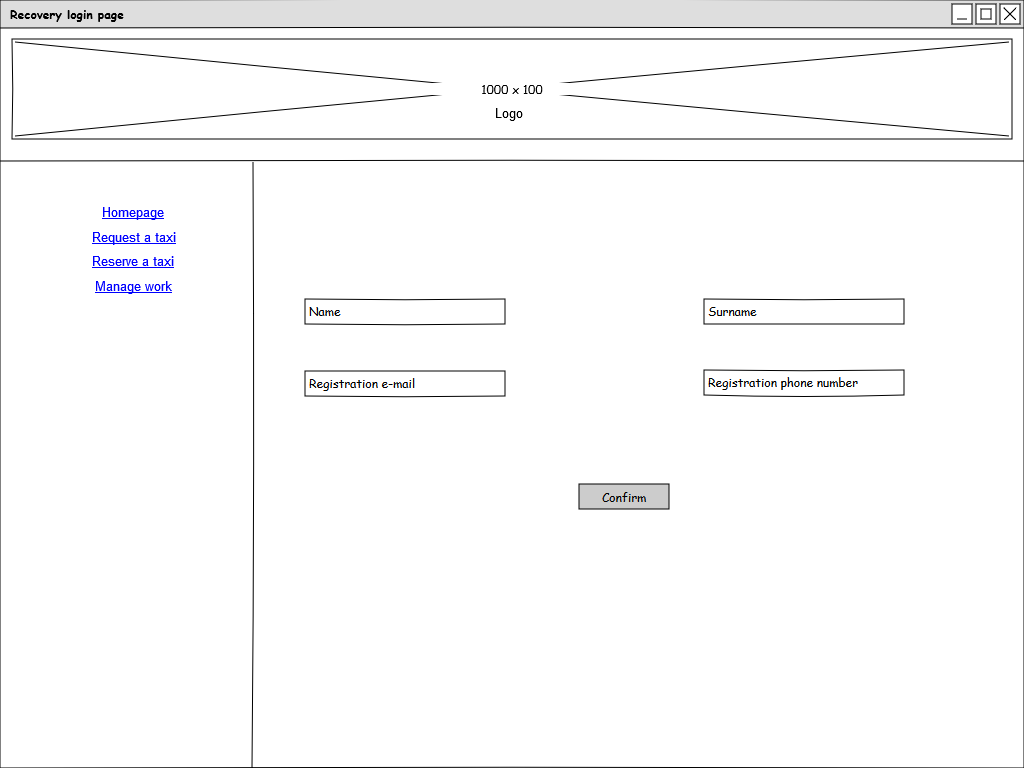
\includegraphics[scale=0.35]{mockups/recovery_login_page_web.png}
\caption{Recovery Web Version}
\end{figure}
\begin{figure}[H]
\centering
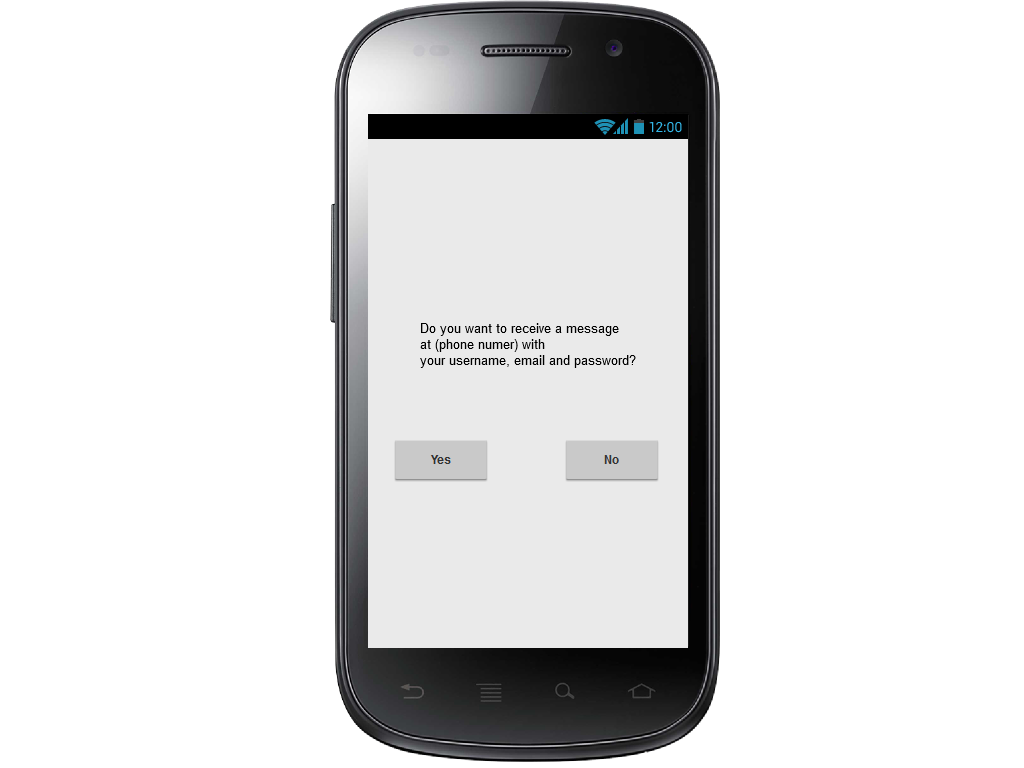
\includegraphics[scale=0.35]{mockups/recovery_login_mobile.png}
\caption{Recovery Mobile Version}
\end{figure}
\break
\subsection{Request}
Both web page and mobile application page show how to request a taxi: in the top field registered passengers have to insert the location where they want to be picked up. This is optional, in fact registered passengers can decide to be geolocalized to be picked up where they are. The map below shows them where the inserted place is or, if they haven't inserted anything, where they are. On the bottom of the page there is another field where registered passengers have to insert the number of passengers who will take that taxi. After compliting all these operations, it is necessary to push ``Confirm'' (for browser) or ``Reserve'' (for mobile application) to send the request to reserve a taxi. \newline As usual, on the left part of the web page there are hyperlinks to reach the most important pages.
\begin{figure}[H]
\centering
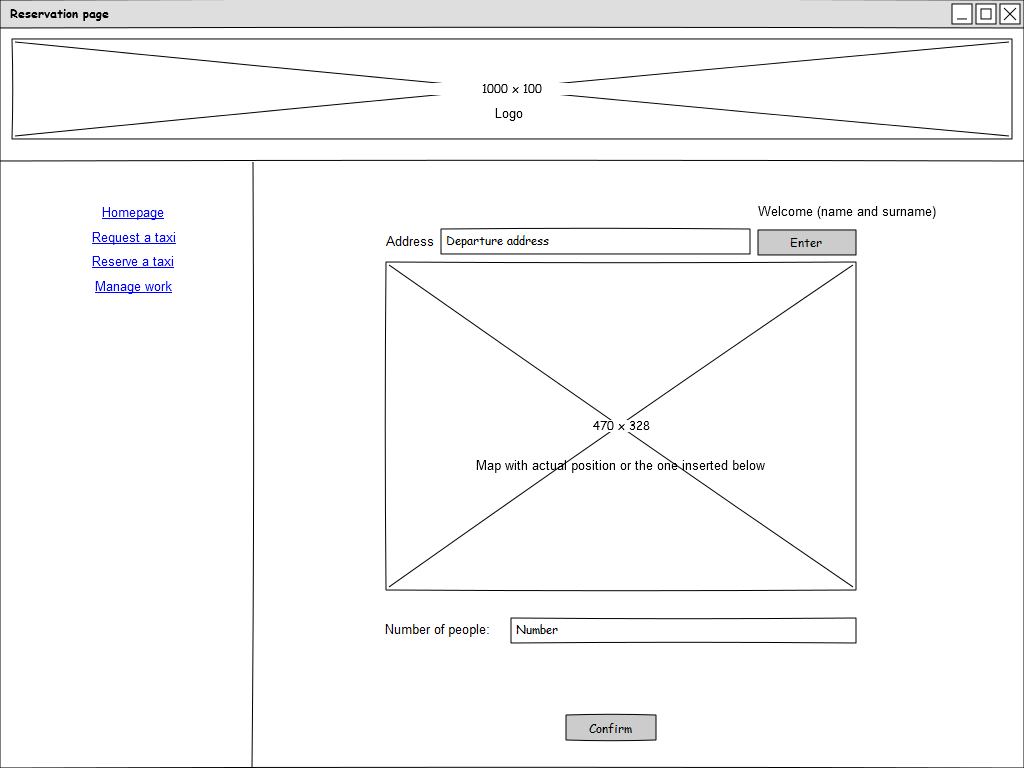
\includegraphics[scale=0.35]{mockups/request_web.png}
\caption{Request Web Version}
\end{figure}
\begin{figure}[H]
\centering
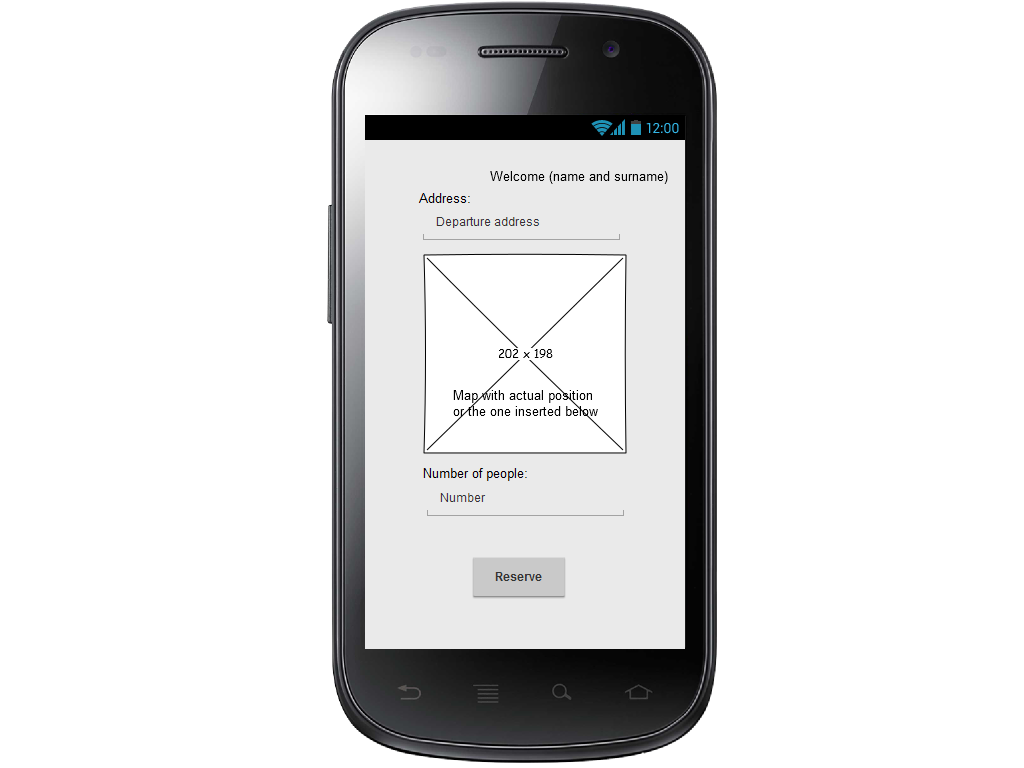
\includegraphics[scale=0.35]{mockups/request_mobile.png}
\caption{Request Mobile Version}
\end{figure}
\break
\subsection{Reservation}
As before, also for reservation, registered passengers have to be geolocalized or they have to insert the location where they want to be picked up and it is mandatory to select the number of passengers. Plus, to make a reservation, it's necessary to select hour and date when passengers want to take a taxi. \newline Also from this browser page users can go to homepage and other important pages. 
\begin{figure}[H]
\centering
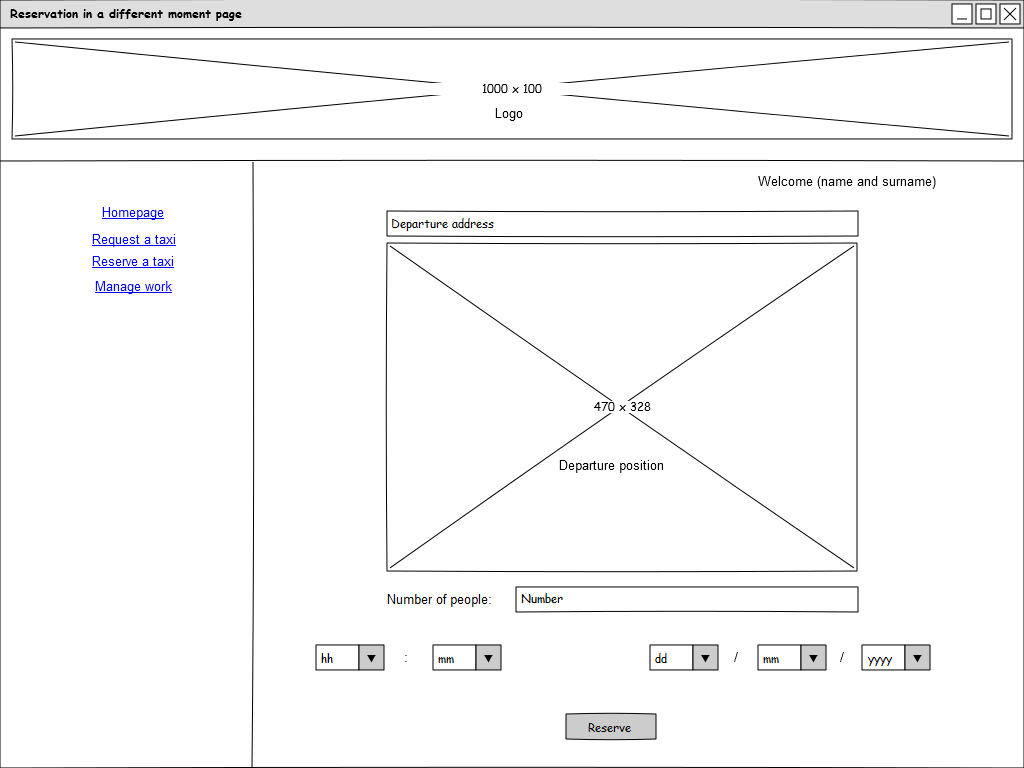
\includegraphics[scale=0.35]{mockups/reservation_web.png}
\caption{Reservation Web Version}
\end{figure}
\begin{figure}[H]
\centering
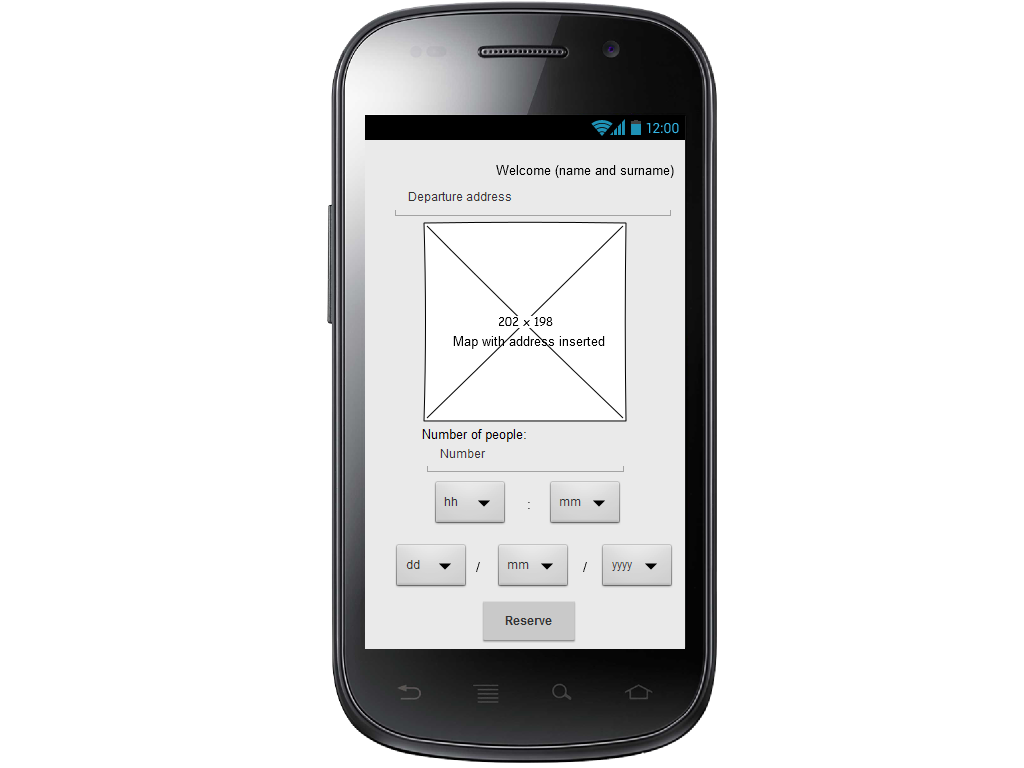
\includegraphics[scale=0.35]{mockups/reservation_mobile.png}
\caption{Reservation Mobile Version}
\end{figure}
\break
\subsection{Driver Interface}
This page is accessible only to registered taxi drivers, here they can manage incoming requests and reservation. Using ``Previous'' and ``Next'' buttons, taxi drivers can select available requests and reservations, accepting or refusing them clicking on specific buttons. For every request and reservation, there is a map that shows to taxi drivers where passengers want to be picked up. \newline As usual, on the left part of the web page there are hyperlinks to reach the most important pages.
\begin{figure}[H]
\centering
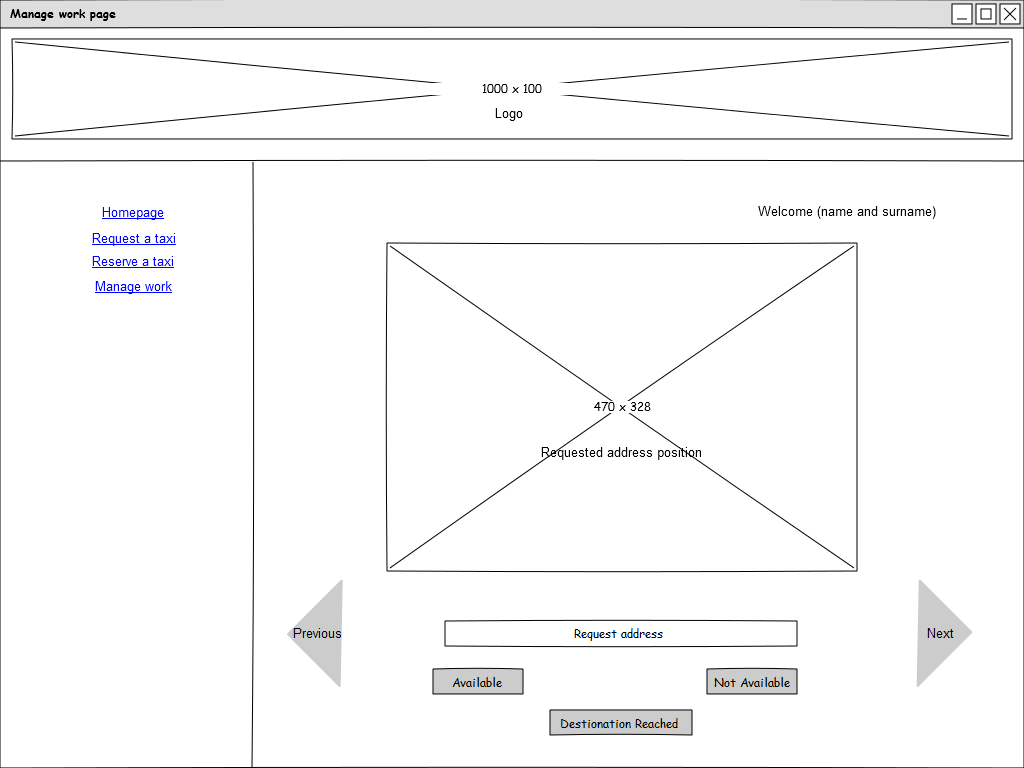
\includegraphics[scale=0.35]{mockups/manage_work_web.png}
\caption{Driver Interface Web Version}
\end{figure}
\begin{figure}[H]
\centering
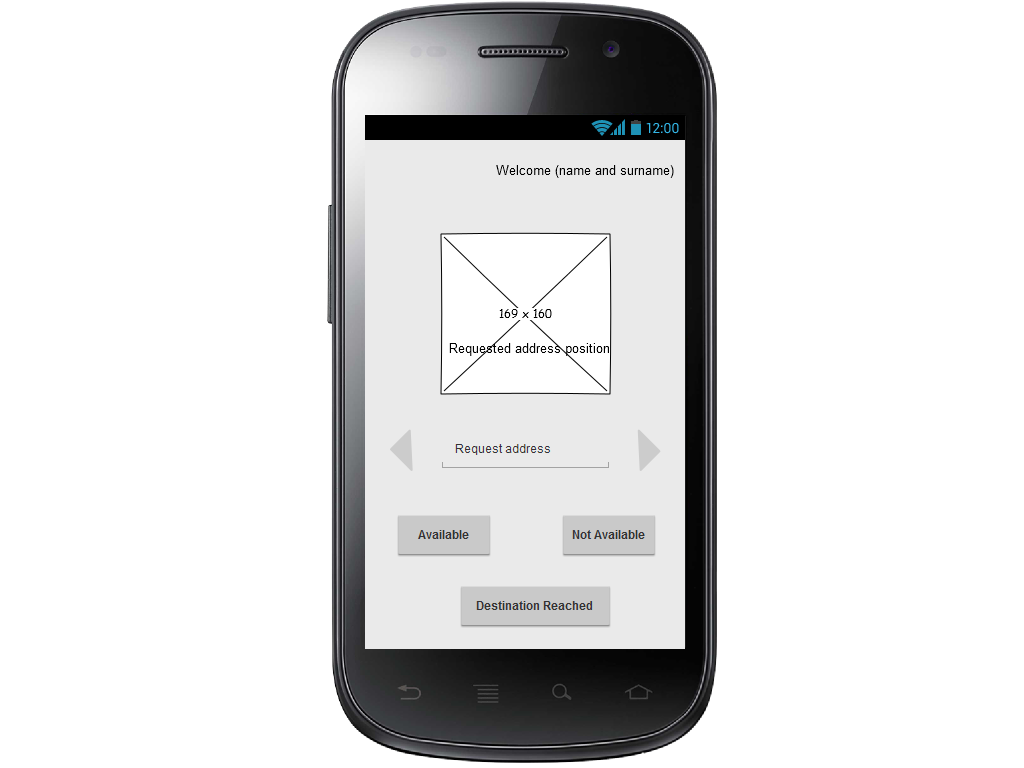
\includegraphics[scale=0.35]{mockups/manage_work_mobile.png}
\caption{Driver Interface Mobile Version}
\end{figure}
\break
\subsection{Administrator}
This page is accessible only to the administrator. He/she has to convalidate, modify, delete taxi driver profiles in case drivers respectively register themselves, change information about them or resign. \newline Hyperlinks work exactly like in other cases, but to use web and mobile functions it's necessary to log in as passengers or taxi driver.
\begin{figure}[H]
\centering
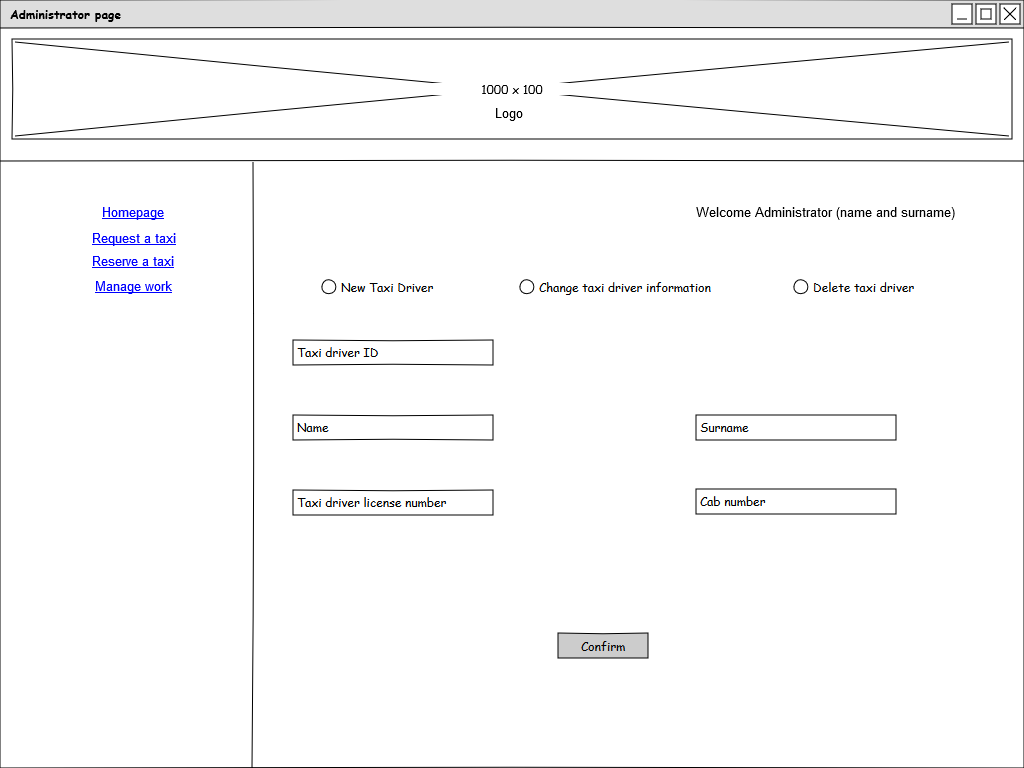
\includegraphics[scale=0.35]{mockups/administrator.png}
\caption{Administrator Web Page}
\end{figure}
